\chapter{The Poisson Problem}

Picture showing a cube, embodying the physical domain, with arrow out to an equation (Laplacian), and then arrows pointing to entries in a matrix from the portions of the equation.

\begin{align}
  -\Delta u =  f
\end{align}

We will use MMS to verify our implementation, which means we assume an exact solution $u^*$ and then calculate the corresponding forcing function $f$ which makes it solve our equation. For example, let
\begin{align}
  u^* = x^2 + y^2.
\end{align}
Then we have
\begin{align}
  -\frac{\partial^2 u^*}{\partial x^2} - \frac{\partial^2 u^*}{\partial y^2} &= f, \\
  -2 - 2 &= f, \\
  -4     &= f.
\end{align}

\section{Variational Formulation}
Consider the poisson strong form on the domain in fig. \ref{Domain},
\begin{figure}[!ht]
\begin{center}
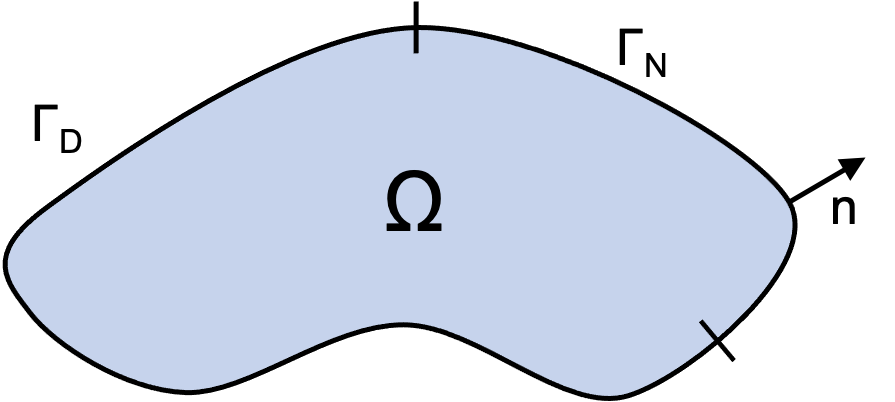
\includegraphics[scale=0.6]{figures/Domain.png}
\end{center}
\caption{General domain for solving}
\label{Domain}
\end{figure}
\begin{align}
-\Delta u &= f \;\; in \;\; \Omega, \\
u &= u_0 \;\; on \;\; \Gamma_D \subset \partial \Omega, \\
\nabla u\cdot n &= g \;\; on \;\; \Gamma_N \subset \partial \Omega.
\label{pde}
\end{align}
To discretize this equation, we use the finite elements method.  The first step in discretization is to derive a weak (or variational) formulation.  The process used to derive the weak form for the poisson equation in this project can be found in \cite{AutomatedFEM2011} and \cite{Fenics2017}.  We start by multiplying by a test function $v$ and integrating over the domain to obtain,
\begin{equation}
-\int_{\Omega} (\Delta u) \, v \, dx = \int_{\Omega} f \, v \, dx.
\end{equation}
It is common when deriving weak formulations to try and reduce the order of the derivatives of $u$ and $v$ as much as possible.  In the case of the poisson equation, the laplacian term can be reduce to two first order gradients of $u$ and $v$ using integration by parts.  The integration by parts formula reads,
\begin{align}
-\int_\Omega (\Delta u) \, v \, dx &= \int_\Omega \nabla u \cdot \nabla v - \int_{\Gamma} \frac{\partial u}{\partial n} \, v \, ds, \\
 &= \int_\Omega \nabla u \cdot \nabla v - \int_{\Gamma} \nabla u \cdot v \, ds,
\end{align}
where $\frac{\partial u}{\partial n} = \nabla u \cdot n$ is the derivative of $u$ in the normal direction $n$ on the boundary.  We note that Gauss' Theorem is used to replace the volume integral with the surface integral.  Using this formula on the poisson equation gives,
\begin{equation}
\int_{\Omega} \nabla u \cdot \nabla v \, dx - \int_{\Gamma_N} v \, (\nabla u \cdot n) \, ds = \int_{\Omega} f \, v \, dx.
\end{equation}

Another common rule when deriving weak formulations is that the test function $v$ vanishes on the parts of the boundary where the solution $u$ is known.  This requirement is explained in detail in \cite{Langtangen2019}.  Presently, this means $v=0$ on the entire boundary $\partial \Omega$ simplifying the weak form to,
\begin{equation}
\int_{\Omega} \nabla u \cdot \nabla v \, dx = \int_{\Omega} f \, v \, dx.
\end{equation}
We require that this formulation holds true for all test functions $v$ in some \textit{test space} $\hat{V}$.  From this requirement, we can then determines a unique solution $u$ which lies in some function space $V$, also called a \textit{trial space}.  For this problem, the test and trial spaces, $V$ and $\hat{V}$, are defined as,
\begin{align}
V = \lbrace v \in H^1 (\Omega) : v=u_0 \; on \; \partial \Omega \rbrace, \label{TrialSpace} \\
\hat{V} = \lbrace v \in H^1 (\Omega) : v=0 \; on \; \partial \Omega \rbrace, \label{TestSpace}
\end{align}
where $H^1 (\Omega)$ is the well-known Sobolev space containing the functions $v$ such that $v^2$ and $|\nabla v|^2$ have finite integrals over $\Omega$.  Therefore, the continuous solution of the poisson PDE must lie in a function space where the derivatives are also continuous, however the Sobolev space $H^1 (\Omega)$ allows functions with discontinuous derivatives.  This weaker continuity condition of $u$ in the weak formulation allows the use of piecewise polynomial function spaces, or simply put function spaces constructed by stitching together polynomial functions on simple domains such as intervals (1D), triangles (2D) or tetrahedrons (3D).

The next step is to replace the infinite-dimensional function spaces $V$ and $\hat{V}$ with discrete (finite-dimensional) trial and test spaces $V_h \subset V$ and $\hat{V}_h \subset \hat{V}$.  We define the discrete form of $u$, $u_h \in V_h \subset V$ and plug it back into the variational formulation which gives the discretretized weak form,
\begin{equation}
\int_{\Omega} \nabla u_h \cdot \nabla v \, dx = \int_{\Omega} f \, v \, dx \;\; \forall v \in \hat{V_h} \subset \hat{V}.
\end{equation}
This discretized weak form along with suitable definitions of the discrete trial and test spaces $V$ and $\hat{V}$ define the approximate numerical solution for the poisson equation.  We assume that we have a basis $\lbrace \phi_j \rbrace^N_{j=1}$ for $V_h$ and a basis $\lbrace \hat{\phi}_i\rbrace^N_{i=1}$ for $\hat{V}_h$, where N is the dimension of the space $V_h$.  We can then make an ansatz for $u_h$ in terms of the basis functions of the trail space,
\begin{equation}
u_h (x) = \sum^N_{j=1} U_j \phi_j(x),
\label{ansatz}
\end{equation}
where $U \in \mathbb{R}^N$ is the vector of defrees of freedom to be computed \cite{AutomatedFEM2011}.  Plugging the bases into the variational form gives,
\begin{equation}
\sum^N_{j=1} U_j \int_{\Omega} \nabla \phi_j \cdot \nabla \phi_i \, dx  = \int_{\Omega} f \, \phi_i \, dx \;\;\; i = 1,2,...,N.
\end{equation}

Therefore,a finite element solution $u_h (x) = \sum^N_{j=1} U_j \phi_j(x),$ can be computed for this system by solving the linear system,
\begin{equation}
A U = b
\end{equation}
where,
\begin{align}
A_{ij} &= \int_{\Omega} \nabla \phi_j \cdot \nabla \phi_i \, dx \\
b_i &= \int_{\Omega} f \, \phi_i \, dx.
\end{align}

\section{Structured Grid}

We can solve a 2D Poisson problem on a structured grid using finite differences in SNES ex5,
\begin{bash}
  ./ex5 -param 0.0 -da_grid_x 21 -da_grid_y 21 -da_refine 6
        -ksp_rtol 1.0e-9 -pc_type mg -pc_mg_levels 4 -snes_monitor -snes_view
\end{bash}
This problem has 1,640,961 unknowns on the fine level, and 8,199,681 nonzeros in the system matrix. In more detail,
\begin{center}
\begin{tabular}{rll}
             & Options                                            & Explanation \\
\hline
\bashinline{./ex5} & \bashinline{-da\_grid\_x 21 -da\_grid\_y 21} & Original grid is 21x21 \\
             & \bashinline{-ksp\_rtol 1.0e-9}                     & Solver tolerance \\
             & \bashinline{-da\_refine 6}                         & 6 levels of refinement \\
             & \bashinline{-pc\_type mg}                          & 4 levels of multigrid \\
             & \bashinline{-pc\_mg\_levels 4}                     & \\
             & \bashinline{-snes\_monitor -snes\_view}            & Describe solver
\end{tabular}
\end{center}

\section{Variable Coefficient}

We will introduce a coefficient $\kappa$ into our equation.
\begin{align}\label{eq:poissonVariable}
  -\nabla \cdot \kappa \nabla u = f
\end{align}
Physically, this coefficient can be a diffusivity, or thermal conductivity, or electric permittivity. When $\kappa$ varies in space, we have an extra term in our equation
\begin{align}
  -\nabla \cdot \kappa \nabla u &= f \\
  - \kappa \Delta u - \nabla \kappa \cdot \nabla u &= f
\end{align}
If we want to model a discontinuous coefficient, let us start with a continuous approximant
\begin{align}
  \kappa &= 1 + (\alpha - 1)/2 \left(1 + \tanh\left(\beta \left(x - \frac{1}{2}\right)\right)\right) \\
  \frac{\partial\kappa}{\partial x} &= \frac{\alpha-1}{2} \beta \sech^2\left(\beta \left(x - \frac{1}{2}\right)\right)
\end{align}
so that our equation becomes
\begin{align}
  - \kappa \Delta u - \frac{\alpha-1}{2} \beta \sech^2\left(\beta \left(x - \frac{1}{2}\right)\right) \frac{\partial u}{\partial x} &= f
\end{align}
As $\beta\to\infty$, the transition region shrinks, it is roughly of size $2/\beta$, so that the coefficient looks constant in the left (1) and right ($\alpha$) halves of the domain and the derivative tends toward a delta function of strength $\alpha-1$ at $x = 1/2$. The moral is that form we use for finite elements Eq.~\ref{eq:poissonVariable} will look like the prior equation with constant coefficient, plus a jump term proportional to the normal derivative of the solution where the coefficient changes.

Since we are interested in large coefficient changes, we will set the value of $\kappa = 10^{-k}$, where \bashinline{-k <k>} is the command line argument. We will have three coefficient distributions in our tests. First, the constant distribution. Second, a step function at $x = 0.5$ which is one to the left and $10^{-k}$ to the right. Third, a checkerboard pattern alternating between one and $10^{-k}$. The number of squares per dimension $m$ is set using \bashinline{-div <m>}.
\begin{center}
\begin{tabular}{cl}
$\kappa$  & Option \\
\hline
$10^{-k}$ &\bashinline{-coeff_type constant} \\
1 + $(10^{-k} - 1) \Theta_x(0.5)$ &\bashinline{-coeff_type step} \\
$\left(\lfloor m x \rfloor + \lfloor m y \rfloor\right) \bmod 2 + 10^{-k} \left(\lfloor m x \rfloor + \lfloor m y \rfloor + 1\right) \bmod 2$ &\bashinline{-coeff_type checkerboard} \\
\end{tabular}
\end{center}

We can also introduce a tensor coefficient
\begin{align}
  -\nabla \cdot \boldsymbol\kappa \cdot \nabla u = f.
\end{align}
For our problem, we will restrict the tensor coefficient to diagonal tensors. Thus in 2D we have
\begin{align}
  -\mqty(\partial_x & \partial_y) \cdot \mqty(\alpha & 0\\ 0 & \beta) \cdot \mqty(\partial_x \\ \partial_y) u &= f \\
  -\mqty(\partial_x & \partial_y) \cdot \mqty(\alpha\partial_x \\ \beta\partial_y) u &= f \\
  -\left(\alpha\partial^2_x + \beta\partial^2_y\right) u &= f
\end{align}
and our weak form becomes
\begin{align}
  \left(\nabla v, \boldsymbol\kappa \cdot \nabla u\right) = \int \nabla v \cdot \mqty(\alpha\partial_x u_0 \\ \beta\partial_y u_1)
\end{align}

\section{Unstructured Grid}

We can solve a 2D Poisson problem on a unstructured grid using finite elements in the \bashinline{poisson.c} code in our project. By default, we use \cinline{DMPlexCreateBoxMesh()}, which makes a small structured mesh of a box using either simplicies or tensor product cells. The user can set the cell type, domain dimensions, periodicity, and number of divisions from the command line. After the mesh is created, it can be regularly refined $n$ times using \bashinline{-dm_refine n}. The polynomial degree $k$ for approximation of the potential is set using \bashinline{-potential_petscspace_degree k}.

\section{Visualization}

We can visualize the grid using either X-Windows
\begin{bash}
  ./poisson -dm_refine 2 -potential_petscspace_degree 1 -dm_view draw -draw_pause 2
\end{bash}
or Paraview
\begin{bash}
  ./poisson -dm_refine 2 -potential_petscspace_degree 1 -dm_view hdf5:sol.h5
  ${PETSC_DIR}/lib/petsc/bin/petsc_gen_xdmf.py sol.h5
\end{bash}
The coefficient can also be seen in the same way
\begin{bash}
  ./poisson -dm_refine 2 -potential_petscspace_degree 1 -kappa_view draw -draw_pause 2
\end{bash}
or Paraview
\begin{bash}
  ./poisson -dm_refine 2 -potential_petscspace_degree 1 -dm_view hdf5:sol.h5 -kappa_view hdf5:sol.h5:hdf5_viz:append
  ${PETSC_DIR}/lib/petsc/bin/petsc_gen_xdmf.py sol.h5
\end{bash}
Notice that we have to give the \bashinline{hdf5_viz} format to the $\kappa$ vector since it is local. Global vectors, like the solution, choose this format automatically. We can choose the step function distribution, both from high to low
\begin{bash}
  ./poisson -dm_refine 2 -potential_petscspace_degree 1 -coeff_type step -k 3 -kappa_view draw -draw_pause 2
\end{bash}
and low to high
\begin{bash}
  ./poisson -dm_refine 2 -potential_petscspace_degree 1 -coeff_type step -k -3 -kappa_view draw -draw_pause 2
\end{bash}
We can choose a checkerboard of 64 squares with values 1 and 1000 using
\begin{bash}
  ./poisson -dm_refine 2 -potential_petscspace_degree 1 -coeff_type checkerboard -k -3 -div 8 -kappa_view draw -draw_pause 2
\end{bash}
and a randomized version
\begin{bash}
  ./poisson -dm_refine 2 -potential_petscspace_degree 1 -coeff_type checkerboard -k -3 -div 8 -k_random
    -dm_view hdf5:sol.h5 -kappa_view hdf5:sol.h5:hdf5_viz:append
\end{bash}

\section{Scaling}

We will begin our scaling runs with GMG, but also include AMG eventually. Our first run will use
\begin{center}
\begin{tabular}{ll}
  Options                                                & Explanation \\
\hline
 \bashinline{-potential\_petscspace\_degree 1}           & $P_1$ finite elements \\
 \bashinline{-dm_plex_box_faces 16,16}                   & Original grid is 16x16 \\
 \bashinline{-ksp\_type cg}                              & Use Conjugate Gradients \\
 \bashinline{-ksp\_rtol 1.0e-10}                         & Krylov tolerance \\
 \bashinline{-dm\_refine\_hierarchy 6}                   & 6 levels of refinement \\
 \bashinline{-pc\_type mg}                               & 6 levels of multigrid \\
 \bashinline{-mg\_levels\_ksp_max_it 2}                  & V(2,2) cycle \\
 \bashinline{-mg\_levels\_esteig\_ksp\_type cg}          & Use CG for eigen-estimation \\
 \bashinline{-mg\_levels\_esteig\_ksp\_max\_it 10 }      & Use 10 iterates to estimate the spectrum bounds \\
 \bashinline{-mg\_levels\_ksp\_chebyshev\_esteig 0,0.05,0,1.05} & Chebyshev safety margins \\
 \bashinline{-mg\_levels\_pc\_type jacobi}               & Use Jacobi since it is parallel and GPU friendly \\
 \bashinline{-snes\_monitor -ksp\_monitor -snes\_view}   & Describe solver
\end{tabular}
\end{center}
I notice that my Apple also likes \bashinline{-malloc_debug 0}. Looking at the output of \bashinline{-log\_view}, the total time to solve this system of 1M unknowns on my Macbook is a about 40s, but onyl about 27s is used by the solver itself. Most of the other time is used in the mesh hierarchy setup, such as preallocating the operator and constructing the maps between meshes.

\section{Convergence}

Suppose that we start with the scalable solver above, and wish to look at the convergence of the solver. We will start with a smaller problem of size 16129, where the size is controlled by the number of refinements, using \bashinline{-dm\_refine\_hierarchy 3}. If we use \bashinline{-ksp_monitor}, we can print the residual norm at each iterate. Here an iterate means one V-cycle, and we are using V(2, 2) meaning two Chebhyshev/Jacobi iterations for each smoother application.
\begin{bash}
0 KSP Residual norm 1.246687667754e+02
1 KSP Residual norm 1.173183807978e+00
2 KSP Residual norm 2.148547148913e-01
3 KSP Residual norm 4.363569022569e-02
4 KSP Residual norm 5.269255735305e-03
5 KSP Residual norm 9.652538049515e-04
6 KSP Residual norm 1.407786924015e-04
7 KSP Residual norm 1.857771028731e-05
8 KSP Residual norm 3.107505106987e-06
9 KSP Residual norm 5.461746383081e-07
10 KSP Residual norm 9.885122430428e-08
11 KSP Residual norm 1.740238017074e-08
12 KSP Residual norm 2.779256440973e-09
\end{bash}
We can instead plot the residual decrease as a line graph using \bashinline{-ksp_monitor draw::draw_lg}, as shown on the left in Fig.~\ref{fig:residualPlots}. Using just \bashinline{-ksp_monitor draw}, we can plot the residual itself over the domain, as shown on the right in the figure.

\begin{figure}
\centering
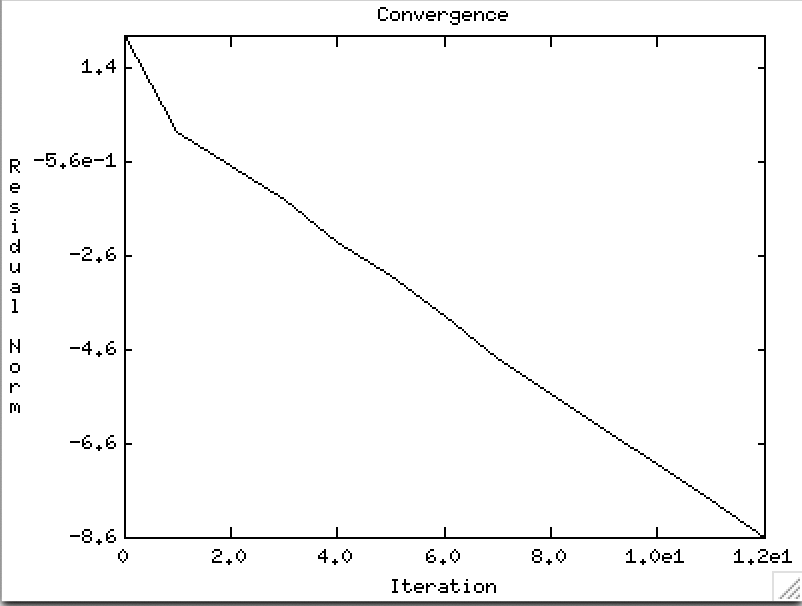
\includegraphics[width=2in]{figures/residualLG.png}\hfil
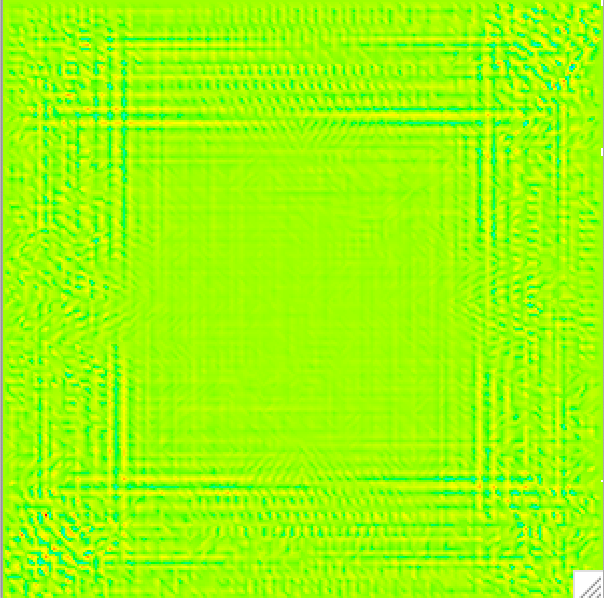
\includegraphics[width=2in]{figures/residualLast.png}
\caption{Plot of residual norm for each iterate of our multigrid solve on the left, and the residual itself for the last iterate on the right\label{fig:residualPlots}}
\end{figure}

The same sequence can be repeated for the error, since we are using MMS and can produce the exact solution. Using \bashinline{-ksp_monitor_error}, we produce the error norm for each iterate.
\begin{bash}
0 KSP Error norm 9.947802867762e-01
1 KSP Error norm 1.000114579455e-02
2 KSP Error norm 1.628832514084e-03
3 KSP Error norm 5.600031707378e-04
4 KSP Error norm 1.947734270258e-04
5 KSP Error norm 2.221932067247e-04
6 KSP Error norm 2.171843316734e-04
7 KSP Error norm 2.176959633670e-04
8 KSP Error norm 2.176494135621e-04
9 KSP Error norm 2.176509954453e-04
10 KSP Error norm 2.176519724470e-04
11 KSP Error norm 2.176516886193e-04
12 KSP Error norm 2.176517676049e-04
\end{bash}
Notice that the error stagnates well before we achieve convergence in the residual. This is because we hit the discretization error for our mesh. Refining the mesh will lower this bound, as we can see by running with \bashinline{-dm_refine_hierarchy 6},
\begin{bash}
0 KSP Error norm 9.993487701143e-01
1 KSP Error norm 1.232700481821e-02
2 KSP Error norm 2.400433256734e-03
3 KSP Error norm 4.230977361349e-04
4 KSP Error norm 6.442041832235e-05
5 KSP Error norm 1.421221753837e-05
6 KSP Error norm 2.668522964351e-06
7 KSP Error norm 3.579243209530e-06
8 KSP Error norm 3.382570470325e-06
9 KSP Error norm 3.409974576211e-06
10 KSP Error norm 3.408023096618e-06
11 KSP Error norm 3.407773635368e-06
12 KSP Error norm 3.407899220660e-06
\end{bash}
As before we can also run using \bashinline{-ksp_monitor_error draw::draw_lg} to generate a line graph of the above sequence, and \bashinline{-ksp_monitor_error draw} to plot the error over the domain, which are shown in Fig.~\ref{fig:errorPlots}. Notice that the error follows the structure of the solution, whereas the residual is much more oscillatory and seems not to be connected to the solution structure.

\begin{figure}
\centering
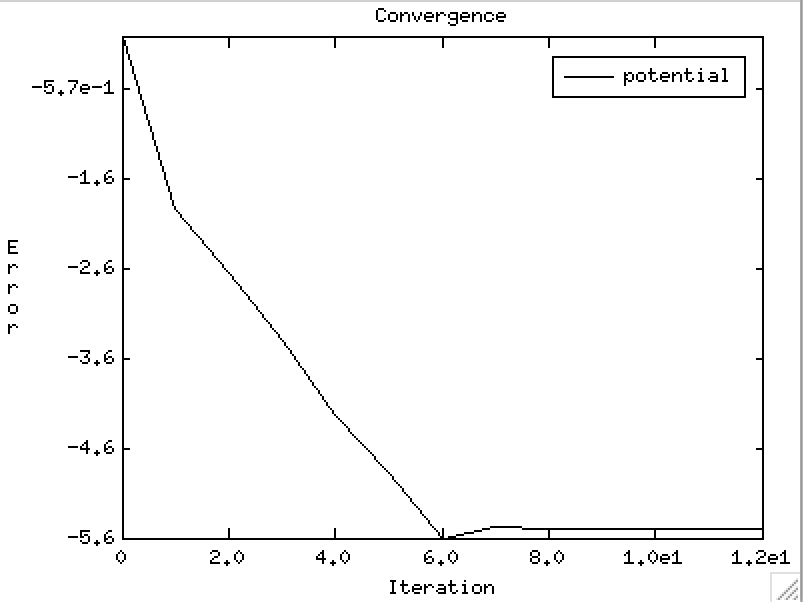
\includegraphics[width=2in]{figures/errorLG.png}\hfil
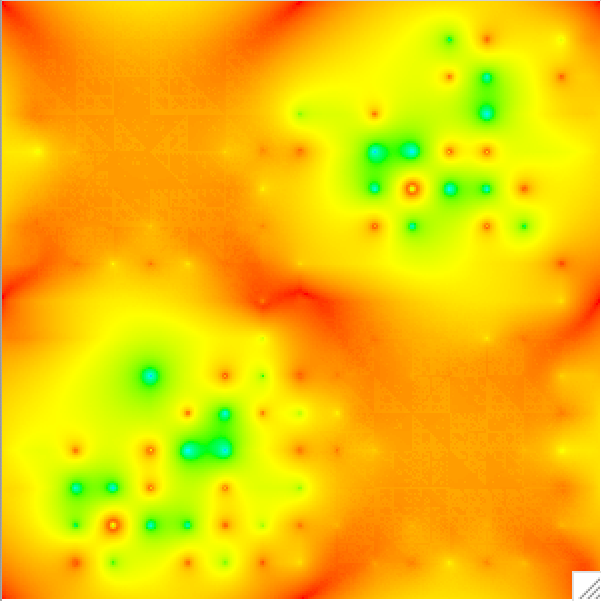
\includegraphics[width=2in]{figures/errorLast.png}
\caption{Plot of error norm for each iterate of our multigrid solve on the left, and the error itself for the last iterate on the right\label{fig:errorPlots}}
\end{figure}
